\providecommand{\PushA}{\frac{5422587}{6103515625}}
\providecommand{\PushExponent}{\frac{5422587}{433349609375}}
\providecommand{\PushDecimal}{1.25131923109859\ldots\cdot10^{-5}}
\providecommand{\PushK}{890666}
\providecommand{\PushTheta}{0.99999999997327}
\section{Introduction}\label{sec:intro}

\subsection{Statement and Context}\label{subsec:intro:statement}

We say that a set $A\subseteq[N]$, where $[N]=\{1,\ldots,N\}$, is
\emph{square-difference-free} if no difference of two distinct elements of
$A$ is the square of a positive integer. Let $s(N)$ be the largest possible
size of such a set. Furstenberg \cite{Furstenberg77} and
S\'ark\"ozy \cite{Sarkozy78} proved that $s(N)=o(N)$. The quantitative
bounds were subsequently improved by Pintz--Steiger--Szemer\'edi
\cite{PSS88} and Bloom--Maynard \cite{BloomMaynard}. Green and Sawhney
\cite{GreenSawhney} then showed that
$s(N)\ll N\exp(-c_0\sqrt{\log N})$ for an absolute $c_0>0$, which
saves more than every fixed power of $\log N$ but less than a fixed
power of $N$. OpenAI \cite{OpenAI} then gave the first power saving,
proving that for some absolute $\eps>0$ we have
$s(N)\le CN^{1-\eps}$.

For the parameter choices displayed in OpenAI's paper, we calculate
(\cref{app:openai-constant})
\[
  \eps\approx10^{-10^{10^{5782.77}}},\qquad\text{in the sense that}\qquad
  \log_{10}\log_{10}\log_{10}(1/\eps)\approx5782.77.
\]
This quantifies that one choice of parameters; it is not a claim
about the best exponent their method could give.

This paper works within the OpenAI framework, and makes $\eps$
explicit, with new quantitative work at almost every step.

\begin{theorem}\label{thm:main}
For every integer $N\ge1$ and every square-difference-free set
$A\subseteq[N]$,
\[
  |A|\le CN^{1-\eps},\qquad
  \eps=\FourRoutesExponent,
\]
so that the exponent is $1-\eps=0.999987\ldots$, where $C$ is
an absolute constant.
\end{theorem}

Here $\eps=a/(72-\vartheta)$ with $a=\FourRoutesA$ and
$\vartheta=\FourRoutesDensity$.

The exponent $1-\eps$ is still far from the exponents in the known
constructions of large square-difference-free sets. Ruzsa's construction
\cite{Ruzsa84}, improved in \cite{BeigelGasarch,Lewko15}, gives
exponents near $0.7334$, and Krachun \cite{Krachun} gave an
exponent exceeding $3/4$. The strongest lower-bound construction
is Naslund's, with exponent $0.7580758$
\cite{NaslundHexagon2026}; its finite certificates are formalized
in Lean \cite{NaslundPalomar2026}.

The shape of the argument is as follows: let $\alpha=|A|/N$ be the density and let $Y$ be the
$72$-point Fourier average defined in \cref{subsec:intro:method}
below. The proof shows $\alpha^{72}\le Y$ (by reflection positivity)
and $Y\le C\Lsc^{-a}\alpha^{\vartheta}$, where $\Lsc=N/\Kint$ is the length of each of the
$\Kint$ subintervals of $[N]$ (Step~1 below). Hence
$\alpha^{72-\vartheta}\ll\Lsc^{-a}$, which is the power saving. Here
$a$ measures decay with scale and $\vartheta$ is the power of
$\alpha$ in the upper bound; for $0<\alpha<1$ a larger $\vartheta$
gives a smaller upper bound at fixed $a$. The word \emph{slot} means
one of the $72$ positions at which the Fourier series is evaluated;
a \emph{law} is a probability or signed distribution on assignments
of group elements to the slots. Full definitions are in
\cref{sec:mechanism} (informally) and Parts~II--III (formally), and
\cref{subsec:intro:glossary} collects the terminology in one place.

The paper proves the upper bound in two stages that share the same
notation and must not be confused. The \emph{baseline} stage, through
\cref{sec:closing}, works with $\vartheta=1$ and proves the
proposition below. The \emph{improved} stage,
\crefrange{sec:density:moments-prefix}{sec:four-routes-closing}, then
strengthens the density estimate to
$\vartheta=\FourRoutesDensity>1$, recomputes the prices (defined
in \cref{subsec:intro:method}) at the new parameters, and proves
\cref{thm:main}. Numerical tables before the
improved stage belong to the baseline unless the caption says
otherwise.
\begin{proposition}[The baseline bound, with density exponent $\vartheta=1$]\label{thm:baseline}
For an absolute constant $C_0$,
$s(N)\le C_0N^{1-\PushExponent}$. This uses $a=\PushA$,
$\vartheta=1$ and $K=\PushK$ intervals (the number $\Kint$ of
intervals in Step~1 below).
\end{proposition}
\Cref{subsec:proof-main} proves this baseline. The improved stage
then reproves the closing inequality at
$a=\FourRoutesA$, $K=\FourRoutesK$ and
$\vartheta=\FourRoutesDensity$; it keeps the same $72$ slots, the same
prime ranges and the same middle reference laws. It uses the new upper
comparisons of \cref{subsec:upper-six-refinements}, the joint mean
allocation of \cref{subsec:joint-mean}, the stronger density estimate,
and the prefix law of Step~4 below. No result
before the improved stage depends on $\vartheta>1$.
\Cref{sec:history} (Part~VI, after the proof) records how the
explicit exponent developed; no proof in Parts~I--V uses it.

The rest of this introduction explains the proof
(\cref{subsec:intro:method,subsec:intro:steps}) and what is new in it
(\cref{subsec:intro:new,subsec:intro:deligne}), states the closing
inequality with its baseline values (\cref{subsec:intro:inequality}) and the
kinds of input (\cref{subsec:intro:status}), and ends with a reading
guide (\cref{subsec:intro:outline}). It proves nothing; every statement
in it is proved later.

\subsection{Overview}\label{subsec:intro:method}


\begin{figure}[tp]
\centering
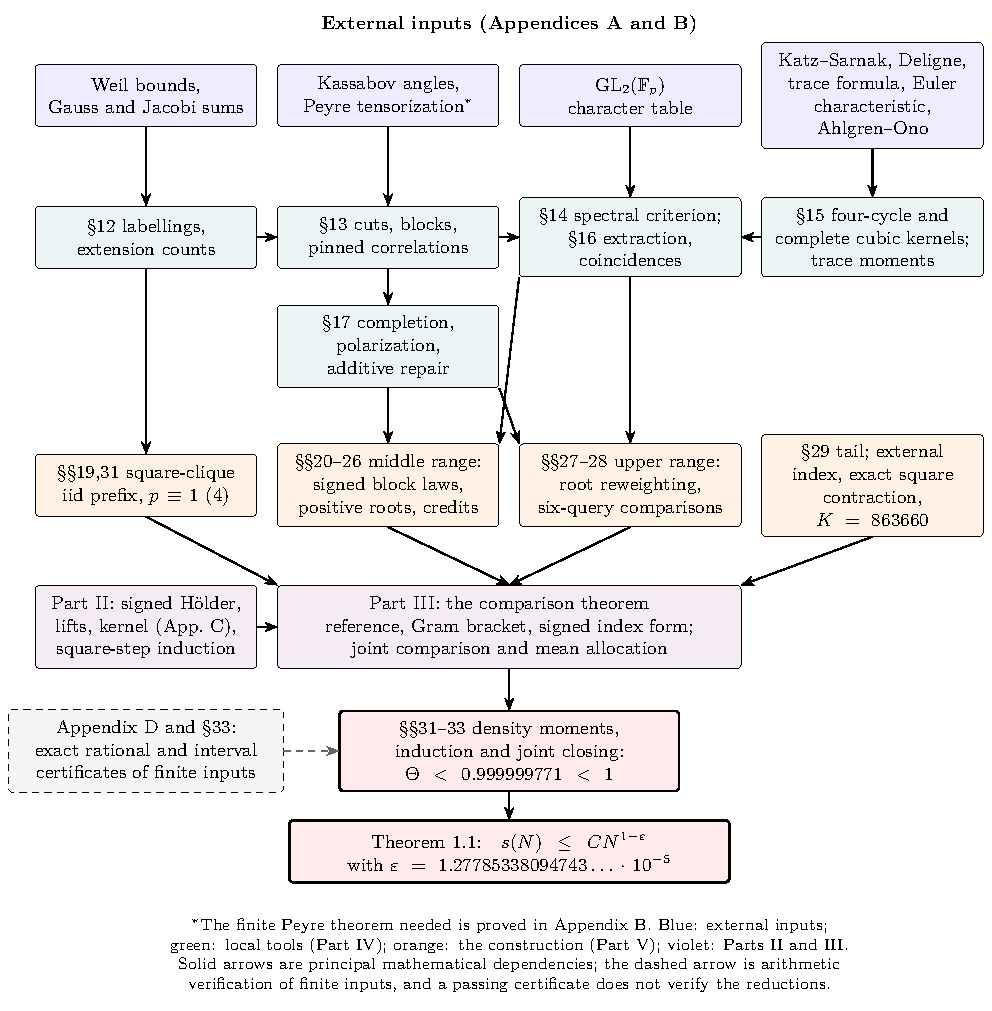
\includegraphics[width=\textwidth]{figures/dependency_graph.pdf}
\caption{Principal dependencies of the proof. External inputs feed the
local tools of Part~IV; these build the laws of the construction in
Part~V, which verify the hypotheses (CP0)--(CP8) of the comparison
theorem of Part~III. The selected density moments and induction extend
the analytic framework of Part~II; the normalized closing in
\cref{sec:four-routes-closing} then gives \cref{thm:main}. The dashed arrow
records finite arithmetic checks, whose scope is stated in
\cref{subsec:intro:status} and \cref{app:certificates}. The parts are
described in \cref{subsec:intro:outline}.}
\label{fig:intro:dependencies}
\end{figure}


The whole proof is organised around one average attached to $A$.
We define it in this subsection, show that it is large when $A$ is
dense, and then explain how the induction proves that it must in
fact be small. The rest of the paper either proves these two bounds
or constructs the distributions that make the second bound explicit.

\paragraph{The average $Y$.}
Write $\alpha=|A|/N$ for the density of $A$, and write
$N=\Kint\Lsc$, where $\Kint$ is a fixed number of intervals and
$\Lsc$ is the scale. There are $72$ \emph{slots}, forming a set $V$
(Step~1 below gives the exact array). A \emph{label} is an element
of a finite group $G_N$ built from residue classes at the primes;
a \emph{configuration} is a choice of one label $z_v$ for each slot
$v\in V$. Let $F_A$ be the truncated Fourier series of $\one_A$ on
$G_N$ (the \emph{Fourier lift} of $A$; see \cref{sec:lifts}). It has
mean $\alpha$, but it may take negative values. Finally, let $\mu$
be a probability distribution on configurations, built as a product
over blocks of primes. We call $\mu$ the \emph{reference law}, and
put
\[
  Y=\E_\mu\prod_{v\in V}F_A(z_v).
\]
Thus $Y$ is a $72$-fold Fourier average of $A$: we choose a random
configuration from $\mu$ and multiply the values of $F_A$ at its
$72$ labels. If $F_A$ were the constant $\alpha$, this would be
exactly $\alpha^{72}$.

\paragraph{Why $Y$ is large.}
The reference law $\mu$ is \emph{reflection positive}: for each of
several mirror symmetries of the slots, the matrix that couples the
two halves of a configuration is positive semidefinite
(\cref{sec:mechanism} informally, \cref{sec:positivity} formally).
Repeated Cauchy--Schwarz across these symmetries gives a signed
H\"older inequality, and hence
\[
  \alpha^{72}\le Y.
\]
The sign of $F_A$ is the point. For a nonnegative function this
would be an ordinary moment bound; here reflection positivity is
what makes the same conclusion available for the signed lift.
In particular, a dense set $A$ forces $Y$ to be large.

\paragraph{What we prove about $Y$.}
Against this, we prove an upper bound of the form
\[
  Y\le C\Lsc^{-a}\alpha^{\vartheta},
\]
where $a>0$ is fixed and $\vartheta=1$ in the baseline argument;
the final argument obtains the stronger exponent
$\vartheta=\FourRoutesDensity>1$. The two bounds together give
$\alpha^{72-\vartheta}\ll\Lsc^{-a}$, which is the power saving in
\cref{thm:main}.

The upper bound is proved by induction on the scale. Suppose it
failed, and look at the smallest scale $\Lsc$ where it could fail;
call this a \emph{least counterexample}. At every smaller scale
the bound is already known, and the whole comparison below takes
place at this one scale, with the smaller scales available as an
induction hypothesis.

\paragraph{Forcing six square differences.}
At a least counterexample we change the reference law $\mu$ into a
law that forces six specified pairs of slots, called
\emph{queries}, to receive labels differing by a square class at
every prime. For such a law the average is negligible compared
with $Y$: roughly, it counts pairs of elements of $A$ at square
distance, and $A$ has none. Making this precise is the kernel
estimate of Step~3 below; it is the only place where the hypothesis
that $A$ is square-difference-free is used directly.

The change of law is made in two stages, $\mu\to\lambda\to\nu$.
The \emph{first-stage law} $\lambda$ is obtained from $\mu$ by a
small number of explicit changes. (A \emph{record} is one weighted
summand in the explicit expansion of a local law; a
\emph{component} of a signed combination is one nonnegative summand
of that combination. The two words are distinct throughout.) The
\emph{comparison law} $\nu$ is a finite signed combination of
nonnegative laws, each of which \emph{accepts} the six queries:
almost surely, each query pair differs by a nonzero square at every
field prime (a prime whose coordinate in $G_N$ is $\Fp$) and by a
nonvanishing square class at the prime-power coordinates, and the
summand has the uniform one-slot marginals required in (CP4).
In informal prose we say such a summand \emph{forces} a square
difference when only the almost-sure square condition is meant;
\emph{accepts} always includes the marginal requirement. Their
formal definitions are (CP1), (CP2) and (CP4) in
\cref{sec:comparison-theorem}.

The law $\nu$ is signed, so it need not be reflection positive,
and the lower-bound argument does not apply to it. It is instead
controlled at one distinguished mirror symmetry $\iota$, the
\emph{reserved cut} (the other symmetries are used for the lower
bound). A positive law $\Nbr$ dominates $\lambda$ at this cut, in
the sense that the block matrix of cut forms
$\bigl(\begin{smallmatrix}\Nbr&\lambda\\
\lambda&\Nbr\end{smallmatrix}\bigr)$ is positive semidefinite
(written $\succeq_\iota0$ below), and a second pair of positive
laws dominates $\nu$ itself. The symmetric and \emph{skew}
(antisymmetric under $\iota$) parts of each change
$\nu-\lambda$ are dominated and priced separately.

\paragraph{What a price is.}
It remains to say what these changes cost. The primes are grouped
into \emph{blocks} $\Blk$; write $q_{\Blk}$ for the product of the
primes in $\Blk$. Fixing the labels at one block fixes a residue
class modulo $q_{\Blk}$, and splitting that class into progressions
with square step restricts $A$ to shorter progressions with square
step (Step~2 below). Those shorter sets
are still square-difference-free, so the induction hypothesis
applies to them. This is the only use of the induction hypothesis,
and its quantitative form is:

\begin{quote}
Changing the law at one block $\Blk$ changes $Y$ by at most
$(\text{size of the change})\times q_{\Blk}^{2a}\times Y$, up to a
factor $1+o(1)$ as $\Lsc\to\infty$.
\end{quote}

The product (size of the change)${}\times q_{\Blk}^{2a}$ is called
the \emph{price} of the change. The ``size'' is a total variation
or an operator norm, according to the kind of change, and norms are
always taken relative to the true one-half distributions of the
record being replaced (its \emph{actual marginals}), not relative
to a product approximation; the three precise forms are in
\cref{def:price} and are summarised in
\cref{subsec:intro:glossary}. Grouping primes into blocks means
the factor $q_{\Blk}^{2a}$ is paid once per block rather than once
per prime. Character sums bound the sizes: they measure how far
the local laws are from independent. The finite certificates of
Part~V then verify that, for one fully specified construction, all
these sizes are small enough; they check finite inequalities only,
not the analytic arguments (\cref{subsec:intro:status}).

So the task of the paper can be stated plainly: construct laws
that are reflection positive where the lower bound needs it, that
force the six square differences where the kernel estimate needs
it, and whose total price is strictly less than $1$. These three
requirements pull against each other, and most of the paper is
about meeting them simultaneously.

\paragraph{The six indices and the number $\Theta$.}
One point has been suppressed. The prime $2$ and the small primes
$p\equiv3\pmod4$ are not coordinates of $G_N$. Each query therefore
also carries an \emph{external index}: an interval number and a
residue modulo a fixed modulus. A signed average over the six
indices expands into $2^6=64$ terms. Every term that couples a
query across two adjacent intervals is negligible by the kernel
estimate, except when the next interval wraps cyclically from the
last interval back to the first; these exceptional terms are the
\emph{wrapping} terms, and they are priced separately.

Collecting the prices of all the changes above gives a single
number, which in the baseline argument is
\begin{equation}\label{eq:intro:closing}
 \Theta=\tfrac{63}{64}\bigl(L_0+\mathcal E\bigr)+J+W+\tfrac{1-m}{64}.
\end{equation}
Here $L_0$ is the total price of the first-stage change
$\mu\to\lambda$; $\mathcal E$ is the total dominated price of the
comparison change $\nu-\lambda$ at the reserved cut; $J$ bounds
the coupled terms coming from the external indices; $W$ bounds
the wrapping terms; and $m>1$ measures how much of the mean
(constant-function) part of $Y$ the dominating laws retain
(\cref{sec:matching-mean}), so the last term $(1-m)/64$ is a
credit. The factor $63/64$ records that the empty term of the
$64$-term expansion is the comparison average itself. All symbols
are defined fully in \cref{subsec:intro:inequality} and
\cref{sec:comparison-theorem}.

If $\Theta<1$, then at a least counterexample the priced upper
bound for $Y$ is incompatible with the lower bound
$\alpha^{72}\le Y$. Hence there is no least counterexample, and
the upper bound holds at every scale. This implication is the
comparison theorem, Theorem~C (\cref{thm:comparison}); its proof
(\cref{sec:comparison-lemmas,sec:comparison-proof}) uses nothing
about the particular local laws, and \cref{prop:mech:one-query}
shows the whole mechanism with a single query. The rest of the
paper verifies the hypotheses of Theorem~C for one explicit
construction and evaluates $\Theta$. For \cref{thm:main} the
improved stage then uses the joint form of this criterion
(\cref{cor:joint-closing}) together with the stronger density
induction; \eqref{eq:intro:closing} is its baseline form.

\paragraph{Why this shape gives a power saving.}
The conversion is worth isolating. Suppose that at some fixed
$a>0$, independent of the scale and of $\alpha$, the construction
above can be priced with $\Theta<1$. Then
$\alpha^{72-\vartheta}\ll\Lsc^{-a}$ at once, so
$\eps=a/(72-\vartheta)$: no iteration is needed, and the saving is
a fixed power for the elementary reason that the required win does
not shrink as $\alpha\to0$. This is also where the quantitative
difficulty lies. With only the first-order (Weil) bounds
$O(p^{-1/2})$ for the local character sums, the best certified
value of $\Theta$ is still larger than $1$
(\cref{subsec:intro:deligne}); the second-order bounds
$O(p^{-1})$ of Part~IV, the relative (actual-marginal) form of the
local estimates, and the variance and mean subtractions are what
bring the total price below $1$ at an explicit value of $a$.

\paragraph{Is this a density-increment argument?}
In ancestry, yes; in form, no. The classical arguments
\cite{PSS88,BloomMaynard} (and \cite{GreenSawhney}) assume that
$A$ is dense and square-difference-free, count square differences
by Fourier analysis, and deduce that $A$ has larger relative
density on a shorter structured set---a progression with square
step in \cite{PSS88}, a Bohr set in \cite{BloomMaynard}. Iterating
this increment until the density would exceed $1$ bounds $\alpha$.
Each step gains only a small factor in density and loses length,
so the final saving is smaller than any fixed power of $N$.

The present proof uses the same square-step rescaling, but it
never produces a denser set. Instead, the induction hypothesis at
all smaller scales is used at once, at a least counterexample, in
the form of prices: passing to the shorter progressions is what
makes a change of law at one block cost the factor
$q_{\Blk}^{2a}$. And the quantity being bounded is not the density
$\alpha$ itself but the $72$-fold average $Y$. This is where the
extra strength comes from. Since $\alpha^{72}\le Y\le
C\Lsc^{-a}\alpha^{\vartheta}$ with $\vartheta\approx1$, a single
constant-factor win---the inequality $\Theta<1$ at one scale---already
gives $\alpha^{72-\vartheta}\ll\Lsc^{-a}$: the $72$ slots amplify
one rescaling gain into a power saving, with no iteration and no
repeated loss of length. The cost of this amplification is that
$F_A$ changes sign, so the positivity that a density has for free
must be manufactured (this is the role of reflection positivity),
and the change of law must be priced in the actual marginals with
second-order character-sum bounds, so that the total price
converges at an explicit value of $a$.

\paragraph{The eleven ingredients, in order of first use.}
The genuine ideas, in the order in which the paper uses them, are:
(i)~reflection positivity across mirror symmetries of the slots;
(ii)~rescaling by progressions with square step, with an induction
linear in the density; (iii)~the kernel estimate of Step~3;
(iv)~handling small primes jointly through one signed external
index per query; (v)~graph laws made reflection positive by adding
correction summands, the principal law itself sometimes reweighted;
(vi)~replacements that keep the true one-half distributions, so
their differences pair to zero with constants and can be bounded by
operator norms; (vii)~controlling a signed, non-positive comparison
law by domination at one cut, with symmetric and antisymmetric
changes bounded separately; (viii)~signed combinations over a whole
block of primes whose first-order change is purely antisymmetric
(adding an edge together with its mirror is the simplest case);
(ix)~subtracting variance and related savings and retaining the
common mean, instead of bounding every term trivially;
(x)~square cliques for the primes $p\equiv1\pmod4$;
(xi)~exact star factorisation: a \emph{star} is a set of cross pairs
sharing one endpoint; for a half law invariant under the
square-affine maps $z\mapsto rz+t$ with $r$ a square unit, its Gram
matrix is computed exactly, so star sums reduce to finite matrix tests.

\paragraph{What is routine verification rather than a new idea.}
The spectral certificates for specific graphs, the matching partitions
and their extraction bookkeeping, the local constants of each prime
range, the block partitions and their degree sums, the completion
weights, the dominator witnesses, the tabulated middle prices, and the
arithmetic that evaluates $\Theta$. They sit
behind lemmas stated once, with the finite inputs in the appendices:
monotone majorants are checked at one endpoint, and polynomials with
nonnegative coefficients are evaluated at upper prices.


\subsection{The proof in five steps}\label{subsec:intro:steps}

The five steps are: (1)~a $72$-fold average at least $\alpha^{72}$;
(2)~rescaling to shorter progressions with square step;
(3)~the kernel estimate, the only use of no square differences;
(4)~local distributions, by prime range; (5)~summing the error
bounds and completing the induction.

\emph{Step 1. A $72$-fold average that is at least $\alpha^{72}$.}
Let $N=\Kint\Lsc$, where $\Kint=\PushK$ is a fixed number of intervals
and $\Lsc$ is the scale. The labels live in the finite group
$G_N=\prod_p\Z/p^{e_p}\Z$, the product over three kinds of primes: the
primes $p\equiv1\pmod4$ below $\Pfour=2^{512}$, with $e_p=2\mcl$ and
$\mcl=8192$; the primes $p\equiv3\pmod4$ in $[Q_3,\Pfour)$, where
$Q_3=19\,951\,586$; and all primes in $[\Pfour,N^{1/20}]$; the last two
kinds have $e_p=1$. The prime $2$ and the primes $p\equiv3\pmod4$ below
$Q_3$ are not coordinates; they enter through the external index of
Step~4. The lift $F_A(z)=\sum_\xi\widehat{\one_A}(\xi)e(z\cdot\xi)$ sums,
over the characters $\xi$ of $G_N$ of conductor at most $N^{1/20}$, the
normalized exponential sums $\widehat{\one_A}(\xi)=N^{-1}\sum_{n\in
A}e(-n\xi)$; it has mean $\alpha=|A|/N$, but it may be negative. The $72$
slots are $V=(\Z/6\Z)^2\times\{0,1\}$: two six-chamber coordinates and a
layer. Given a probability law $\mu$ on labellings $z\colon V\to G_N$, put
$Y=\E_\mu\prod_{v\in V}F_A(z_v)$ (\cref{def:record:functional}).

Reflection positivity says that, at specified cuts of the slots, the
matrix of the two halves is positive semidefinite. Here the cuts are the
three chamber reflections of each six-chamber coordinate and the reserved
cut $\iota$, which flips the layer; their folds sort $V$
(\cref{lem:slot-array}). Repeated Cauchy--Schwarz then gives a signed
H\"older inequality. Unlike an ordinary moment, this still works for
functions that change sign. Reflection
positivity entered through statistical mechanics and constructive field
theory \cite{FrohlichSimonSpencer76,DysonLiebSimon78,FrohlichLieb,FILS,
GlimmJaffe87}; in combinatorics the same positive-semidefinite formalism
underlies graph-homomorphism inequalities and flag algebras
\cite{ConlonLee,HatamiNorine11,Razborov07,LovaszGraphLimits12,
BorgsChayesLovaszSosVesztergombi08}. The finite version needed here is
\cref{thm:holder}. For the reference law
$\mu=\bigotimes_{\Blk}\mu_{\Blk}$ of the construction, a product of laws
on blocks of primes that are reflection positive at all these cuts and
square-affine invariant, it gives $\alpha^{72}\le Y$
(\cref{lem:record:holder}).

\emph{Step 2. Rescaling to shorter progressions with square step.}
Fixing the labels at a block of primes specifies an integer residue
class. Splitting it into progressions of square step rescales the
problem to a shorter interval while preserving square-difference
avoidance; the step is the least square divisible by the modulus
(\cref{lem:record:fibre-scale}). The errors in this comparison are
controlled in \cref{sec:lifts,sec:scale-comparison}. At a least
counterexample to $Y\le C\Lsc^{-a}\alpha$ (a smallest scale where
the bound fails, so it holds at every smaller scale) this gives the
prices of \cref{subsec:intro:method}: each slot contributes a factor
$(q_{\Blk}^2)^{a/72}$, hence $q_{\Blk}^{2a}$ over $72$ slots, times
the size of the change at $\Blk$. The moment bounds are linear in $\alpha$, so the
induction keeps the full density factor: from
$\alpha^{72}\le Y\le C\Lsc^{-a}\alpha$ one obtains $\alpha\le C'N^{-a/71}$,
which is the conversion $\eps=a/71$ (\cref{thm:record:lineardensity}).

\emph{Step 3. The kernel estimate: the only use of no square differences.}
Suppose two slots are placed in adjacent intervals and, at every
prime, their labels are forced to differ by a square class. Then the
corresponding Fourier average is negligible: roughly, it counts
pairs from $A$ at square distance, and $A$ has none. Making this
precise is a circle-method calculation with a kernel supported on
squares, for Fourier frequencies up to $N^{1/20}$
(\cref{sec:kernel,app:kernel20}). This is the only step that
directly uses the defining property of $A$. Everything else in the
proof is about arranging, at small price, that six such forced
pairs occur.

\emph{Step 4. Local distributions, by prime range.}
No single elementary estimate is efficient for every prime, and the class
of $p$ modulo $4$ matters. If $p\equiv1\pmod4$, then $-1$ is a square and
the strict-square relation $y-x\in\Qsq$ is symmetric. If $p\equiv3\pmod4$,
exactly one of $y-x$ and $x-y$ is a nonzero square, and the relation is a
tournament, the Paley tournament. The construction has five ranges.
\begin{itemize}
\item \emph{The small modulus.} The external modulus is
$\Mzero=2^{129}\prod_{3\le p<Q_3,\,p\equiv3\,(4)}p^{128}$.
Each query carries an index $(b,s)$: an interval number and a
residue modulo $\Mzero$. Its coupled index is $(b+1,s+r)$, where $r$
is a random square residue. Averaging over $r$ by its exact
conductor gives one number $R_I$ per query, which is how the small
primes enter the closing sum
(\cref{lem:imp:padic-envelope,prop:imp:padic-price,sec:tail-index}).
\item \emph{The class-one prefix.} At the primes $p\equiv1\pmod4$ below
$2^{512}$ the labels are drawn conditionally independently from a random
square clique of $\Z/p^{2\mcl}\Z$, a set whose nonzero differences are
even powers of $p$ times unit squares. This law is reflection positive at
every cut and accepts every query except on the event, of mass
$2^{-\mcl}$ at each such prime, that the two endpoint labels of a
query coincide at that prime,
which the comparison law deletes, at a total price below
$8\cdot10^{-69}$ over all these primes
(\cref{sec:frontier:iidprefix}).
\item \emph{The middle range.} The primes $p\equiv3\pmod4$ in
$[Q_3,\Pthree)$, $\Pthree=167\cdot2^{40}$, are grouped into blocks $\Blk$
with $\sum_{p\in\Blk}\log p\le L=570$, in $33$ pieces. Each block carries a
twelve-label law, completed to a reflection-positive law, and the
comparison records built on it; on the seven largest pieces the
principal twelve-label law is reweighted by a nonnegative function
(\crefrange{sec:middle-reference}{sec:matching-mean}).
\item \emph{The upper range.} The primes $p\equiv3\pmod4$ in
$[\Pthree,2^{512})$, in $310$ bands, carry the completed two-layer law on
all $72$ slots, on blocks with $\sum\log p$ at most a band-dependent
bound ($\le886$) (\cref{sec:upper-reference,sec:upper-comparison}).
\item \emph{Large primes.} Every prime $p\ge2^{512}$, of either
class, forms a block by itself, with price of order $p^{-3/2+2a}$,
hence summable (\cref{sec:tail-index}).
\end{itemize}
The middle and upper laws start from a graph law: the uniform law on
labellings of a small graph by distinct labels whose edges are
strict-square constraints. A graph law is not reflection positive at
chamber cuts: its negative cut spectrum, of order $p^{-1/2}$, is
cancelled by adding folds, matchings, merges and constants with weights
in powers of $p^{-1/2}$; this is a \emph{completion}
(\cref{lem:five-type}). The weights are dictated by spectral bounds for
cut operators (\cref{thm:spectral-criterion,subsec:spec:actual-stars}).
Weil's bound controls them
to first order; the second-order control needed in the middle and upper
ranges comes from the bounds of \cref{subsec:intro:deligne}. The
comparison law keeps every summand that already forces the six
square differences, replaces most others by forcing laws with the
same one-half distributions, and deletes the rest; the price of
each replacement is what Step~5 sums.

\emph{Step 5. Summing the error bounds and completing the induction.}
Each changed record of a block contributes its norm, relative to the
actual half marginals, times $q_{\Blk}^{2a}$. On a block of logarithmic
size at most $L$ the factor $q_{\Blk}^{2a}\le e^{2aL}$ is bounded, while
the local errors are those of its least prime. The prices are summed
over each range with exact prime products and sieved counts below
explicit thresholds and the explicit Chebyshev bound of Bennett, Martin,
O'Bryant and Rechnitzer for primes $p\equiv3\pmod4$ above them
(\cref{thm:bmor}; compare the explicit prime-number literature
\cite{RosserSchoenfeld75,PlattTrudgian21}); the sum over the large
primes is bounded by comparison with an integral. A
signed product over the six disjoint queries amplifies the cancellation
of Step~3. The comparison theorem turns the totals into the single number
$\Theta$, and the proof closes because $\Theta<1$
(\cref{subsec:intro:inequality}).

\subsection{What is inherited from the OpenAI preprint, and what is new here}
\label{subsec:intro:new}

The overall architecture---signed functional, square-step comparison,
actual-square kernel, separate treatment of the exceptional
wrapping terms $W$, and induction---is inherited
from \cite{OpenAI}. Its Fourier-lift and density-comparison steps are
descendants of the classical Roth--Gowers density-increment method
\cite{Roth53,Bourgain99,Gowers01,Sanders11,TaoVu06}, but the
reflection-positive functional replaces a single density increment by
an induction on a much larger multilinear average. The explicit
exponent comes from changing the local laws and the accounting at
almost every quantitative interface.

\paragraph{Where the larger exponent comes from.}
In both proofs the final exponent has the form
$\eps=(\text{scale exponent})/(\text{number of slots})$, and two
separate effects make ours larger; they multiply. The first is the
denominator: the displayed OpenAI construction uses
$d=(24!)^{161}$ slots, with $\log_{10}d\approx3830.63$
(\cref{app:openai-constant}), where we use $72$; at an equal scale
exponent this alone gains about $3829$ orders of magnitude. The
second is the numerator. The OpenAI argument does not quantify its
local estimates, and for its displayed parameters the scale
exponent is forced down by its mixing and modulus thresholds,
making $\eps$ triple-exponentially small
(\cref{app:openai-constant}). Here every local law is rebuilt so
that its price can be summed explicitly: relative rather than
absolute graph estimates, primes grouped into blocks of bounded
budget ($\sum\log p\le570$ in the middle range), norms in the
actual marginals, second-order character-sum bounds, and the
variance and mean subtractions. The outcome is that $\Theta<1$
already at $a=\FourRoutesA\approx9.07\cdot10^{-4}$, and hence
$\eps=a/(72-\vartheta)\approx1.28\cdot10^{-5}$. The items below
are the local changes behind this second effect; the most recent
refinements (the joint mean allocation and the cross-weighted
upper reweighting) improve $\eps$ only by a few percent on top.

\begin{description}[leftmargin=2.2em,style=nextline]
\item[Finite rectangle instead of an enormous one]
The displayed OpenAI construction uses $d=(24!)^{161}$ slots. Here
$V=(\Z/6\Z)^2\times\{0,1\}$ has $72$ slots. This alone changes the
conversion $\eps\approx a/d$ by many orders of magnitude. It also leaves
much less room for waste in the local estimates.

\item[Relative, not merely absolute, graph estimates]
A square-constraint graph over $\F_p$ has very small density.
Weil's bound estimates how many labels remain available after some
neighbours are fixed. We divide by the graph's own expected density
before normalising, so the relevant error is relative. This is what lets
the same construction be used at explicit thresholds.

\item[Small primes enter through a coupled external index]
The prime $2$ and the primes $p\equiv3\pmod4$ below the middle threshold
enter a fixed modulus. Instead of
estimating the rare event that all of their residues are simultaneously
good, the proof couples the index of each query with a shifted copy, so
that a selected difference is forced into a nonvanishing square class.
The resulting price factor is the explicit conductor moment
$R_I$. Exact norm envelopes at
successive prime-power depths and the least square step determine its finite
product (\cref{lem:imp:padic-envelope,prop:imp:padic-price}); the original
prime moments remain an efficiently evaluated upper majorant for its
large-prime part (\cref{cor:imp:padic-majorant,lem:index-moments}).

\item[Dependence after fixing labels is bounded as an operator norm]
After some labels are fixed, the remaining labels are not independent.
Kassabov's subspace-angle inequalities \cite{Kassabov} control
dependence between two labels, and Peyre's maximal-correlation theorem
\cite{Peyre} combines these into bounds between sets of labels;
maximal correlation itself goes back to
\cite{Hirschfeld35,Renyi59,AhlswedeGacs76}. The finite form of Peyre's
result needed here (\cref{thm:peyre-finite}) is proved in
\cref{app:peyre}.
These estimates turn a heuristic ``almost independent'' into operator
bounds that can be inserted into the budget.

\item[Completions instead of independence]
Graph laws are not assumed independent across a cut, nor reflection
positive. Their negative cut spectrum is small and explicit, and the
positive corrections of a completion cancel it; the weights satisfy a few
explicit inequalities dictated by the spectral bounds
(\cref{lem:five-type}).

\item[Non-forcing records are replaced or deleted, not bounded by a union bound]
Records of the reference that do not accept the queries are repaired or
deleted, not covered by a union bound over obstructions. Polarization and
additive repairs produce positive records that impose the query
constraints and keep the actual conditional marginals of the records they
replace. A record difference then annihilates constants, and a record of
weight $O(p^{-1/2})$ costs $O(p^{-1})$.

\item[A comparison law that is not reflection positive]
The accepting law is not assumed reflection positive, and in the middle
range it is a signed combination of nonnegative accepting laws. It is
compared with the first stage at one distinguished cut only, where
a positive law dominates it in the $2\times2$ block sense; its
changes are split into symmetric and antisymmetric parts with
separate bounds, the antisymmetric price entering the closing sum
only through $\cosh A$. The cancellation of Step~3 is applied to each
nonnegative product component, so the signs cost only a constant in a
vanishing remainder (\cref{sec:comparison-theorem}).

\item[Signed whole-block laws and positive envelopes]
In the middle range a fold record of the comparison law is a signed
mixture, taken after the products over the primes of a block, of three
positive accepting laws, each repaired to the actual half marginal of the
record it replaces (\cref{def:record:mixture}). Its first-order change
against that record is purely skew: at a prime $p$, a three-arm star of
norm about $1.2732\,p^{-1/2}$ at the parameter $\tlaw=127/500$. The case
$\tlaw=0$ is mirror pairing, which adds to the record the query edge
together with its mirror image under the reserved reflection; its star has
two arms and norm about $\sqrt2\,p^{-1/2}$ (\cref{lem:mirror}). The
variation $1+\tlaw$ of the mixture
does not grow with the number of primes.
Products of two, four or six antisymmetric changes on distinct
blocks are bounded by quantities smaller than the trivial norm
estimate, using positive semidefinite dominating matrices,
averaged over reflections
(\cref{sec:middle-records,sec:envelopes}).

\item[Norms are taken in the marginals of the record being replaced]
Local laws are measured in the true one-half distribution of the
record they replace, not in a product approximation. Leading terms
and remainders (including coincident labels) are bounded
separately, and simultaneous changes on several blocks by a power
series with nonnegative coefficients in those bounds
(\cref{lem:actual-features,lem:middle-comparison-prices,lem:record:record-expansion}).
In the final upper range, extraction is cross-weighted: the conditional
density of the witness labels is retained together with its cover
marginal, rather than bounded separately and multiplied. The resulting
smaller root caps lead to recomputed completion weights on $301$ bands
(\cref{lem:matching:extractionk,subsec:upper-cross-weighted}).

\item[Star-shaped features with exactly computable Gram matrices]
The star features of a square-affine invariant law have exact Gram
matrices, so the leading part of a cut operator is a finite signed matrix
of star incidences, certified by exact positivity tests
(\cref{subsec:spec:actual-stars}). This gives the bound at one
chamber symmetry for the principal middle law, whose leading star
matrix has norm exactly $\sqrt{30}$ (\cref{subsec:middle-l20}), and
several upper-range bounds where old and new star matrices differ
in only a few entries (\cref{sec:upper-comparison,lem:joint-rows}).

\item[Reweighting the principal twelve-label law by a nonnegative function]
On the seven largest middle subranges the principal twelve-label law
(the weight-$1$ summand, called a \emph{root} in Part~V; the word has
nothing to do with square roots) is reweighted, at every prime, by
averages of squares of affine functions of three quartic trace
statistics, or by a $39$-trace square with a positive constant added
(\cref{def:positive-root}). The reweighting keeps the symmetries,
keeps the support inside the accepting set, and improves the
one-sided spectral bound across a chamber symmetry; the changed
one-half marginal is accounted for separately
(\cref{sec:positive-roots}).

\item[Errors are tensored at the cut where they are largest]
The two repaired folded matching records of the first stage attain
their largest cut norms (their sharp prices) at different cuts.
All record differences whose sharp price is attained at one cut
are tensored there, which makes the first-stage error and the
error part of the bracket about sixteen times smaller than a bound
with one sharp factor per term
(\cref{lem:sharp-first,cor:two-cut-series}).

\item[Subtractions in the closing inequality (variance, dominators, mean)]
Three quantities are subtracted (or, for the mean, credited) in
$\Theta$ rather than bounded trivially: the variance saved when a
replacement preserves one-half distributions
(\cref{sec:variance}); the saving from dominating matrices for
products of changes (\cref{sec:envelopes,prop:signed-sides}); and
the common mean energy $m>1$ retained from the six indices
(\cref{sec:matching-mean}). In the final closing, higher mean
contributions are allocated jointly against the same labelled positive
comparison coefficients before upper prices are substituted; only the
residual series with nonnegative coefficients is then completed
(\cref{cor:joint-closing,subsec:joint-mean}). If only the variance and dominator
savings were removed, with all other credits kept, $\Theta$ would
exceed $1$ by about $0.46$ in the baseline; see
\cref{subsec:intro:inequality}.

\item[Improving the power of $\alpha$ in the induction]
The baseline moment bounds are linear in the density, with conversion
$\eps=a/71$. The final argument strengthens this to
$\alpha^{\FourRoutesDensity}$. Most laws are controlled by grouping
labels in pairs; rare cases where many labels coincide are instead
handled by fixing (\emph{pinning}) the coinciding labels and
rescaling the resulting shorter progressions, and a new prefix law
with independent labels
removes repeated-label concentration. These steps are proved after
the baseline closing (\cref{sec:density:moments-prefix} and
\cref{sec:density-upgrade}). The comparison error is bounded before
the operator reduction, and the square-step main term is then
estimated with the actual folded laws and their mixed moments,
as in \cref{prop:density:production}.

\item[A kernel for larger cutoffs]
The actual-square kernel is proved for Fourier cutoffs up to $N^{1/20}$
and for prime-power moduli (\cref{app:kernel20}), so that the class-one
primes can carry labels modulo $p^{2\mcl}$.

\item[Estimates are verified at explicit prime thresholds]
The middle range starts at $Q_3=19\,951\,586$ and the upper range at
$\Pthree=167\cdot2^{40}$. These are not asymptotic placeholders: at the chosen
thresholds, exact rational matrices and interval inequalities verify the
hypotheses of the analytic lemmas, and monotone majorants carry each
check to all larger primes. \Cref{app:certificates} states precisely which
assertions are computational.
\end{description}

\paragraph{The general machinery and the earlier explicit design.}
The first explicit versions of this argument used the slot array
$(\Z/6\Z)^3$, with $216$ slots, and a reserved cut that was a chamber
reflection of the third coordinate. Most of the general machinery of
Parts~II--IV was developed for that $216$-slot design: the chessboard
calculus on products of reflection coordinates; lifts, moments, conductor
decay and the actual-square kernel; the external index and its coupling;
graph laws with Weil-type insertion counts and pinned influence; the
spectral criterion with its coupling block, its witness extraction and the
four-cycle bound; completions by folds, matchings, merges and constants;
and the comparison of three laws, an all-cut reference, an intermediate
law and an accepting law, by polarization and additive repairs that keep
the actual conditional marginals. Parts~II--IV state it once, in the
generality the final design uses. The final proof is that design
re-instantiated on $72$ slots, with new local laws and four structural
substitutions (\cref{tab:walk:substitutions}): a two-point layer whose
flip is the reserved cut replaces the third six-chamber coordinate, which
changes the conversion at the same $a$ from $a/(216-\vartheta)$ to
$a/(72-\vartheta)$, hence to $a/71$ for the density-linear
induction with $\vartheta=1$; six disjoint one-way queries
with a common signed index replace coupled families of amplified edges and
their obstruction covers; the comparison law is not reflection positive,
and is controlled at the reserved cut by a positive $2\times2$
block; and the primes are divided by
their class modulo $4$ into the ranges of Step~4. What the final theorem
does not use are the instances of the $216$-slot design: its particular
laws, constants and certificates, and the proofs of its checkpoints.
\Cref{sec:design-walk} explains each substitution as the answer to a
quantitative failure, and \cref{subsec:history:216} lists what survives of
each part of that design.

\subsection{Where the Deligne bound enters}\label{subsec:intro:deligne}

It is useful to separate first-order and second-order character sums.

For one square constraint, or for counting extensions of one label at a
time, the relevant sums contain one quadratic character of a polynomial
with distinct roots. Weil's bound \cite{Weil48,Weil49,Schmidt76} gives
square-root cancellation: after the normalisations of
\cref{sec:labellings}, the
relative error is $O(p^{-1/2})$. Gauss and Jacobi sums evaluate the
constant Fourier blocks exactly \cite{BerndtEvansWilliams,IrelandRosen}.
These tools suffice for a large part of the construction and already
appear, in a simpler form, in the OpenAI argument.

The difficulty is that the spectral estimates are conditional. One has
fixed part of a graph labelling and must compare the joint law of two
remaining labels with a product law. Errors from two one-variable counts
can correlate. Bounding each separately by $O(p^{-1/2})$ is not enough
for the negative spectral side: several terms must be $O(p^{-1})$ after
normalisation, uniformly in the fixed labels and in the polynomials
arising from the graph. A model sum is
\[
  \sum_{y,z\in\F_p}\chi\bigl(f(y)g(z)(y-z)\bigr),
\]
where $\chi$ is the quadratic character and $f,g$ have controlled
degrees and distinct roots. This is the content of \cref{thm:dl:H2}.

There is no single black box in the proof.
Four algebraic-geometric facts are combined:
\begin{enumerate}[label=(\roman*)]
\item The Grothendieck--Lefschetz trace formula rewrites the character
sum as a trace of Frobenius on compactly supported cohomology.
\item For the family of curves $y^2=f(x)(x-z)$, Katz--Sarnak
\cite{KatzSarnak} identify the relevant sheaf: it is lisse, tame, pure and
geometrically irreducible, with large symplectic monodromy. In elementary
language, as the parameter $z$ moves there is no hidden invariant
direction in which all the errors point the same way.
\item The Grothendieck--Ogg--\v Safarevi\v c formula bounds the
dimension of the cohomology in terms of the degrees and ramification.
This is where the explicit, degree-dependent constant comes from.
\item Deligne's theorem on weights \cite{DeligneWeilI,DeligneWeilII}
bounds the Frobenius eigenvalues. After the normalisations in the
spectral problem, this yields the required $O(p^{-1})$ rather than
$O(p^{-1/2})$.
\end{enumerate}
The precise external statements are isolated in \cref{app:external}
(\cref{thm:prelim:ks}); their conversion into the estimates used by the
local laws is carried out in \cref{sec:dl}. A reader willing to accept
\cref{thm:dl:H2} and the second moments of \cref{sec:dl} as named
character-sum estimates can read the rest of the proof without following
the sheaf argument.

A second, different second-order input concerns the complete bipartite
graph $K_{2,2}$. Its character kernel is invariant under
$\mathrm{PGL}_2(\F_p)$. The character table of $\mathrm{GL}_2(\F_p)$
therefore decomposes it into representation blocks, and Gauss--Jacobi
identities bound those blocks. The resulting normalised estimate is $2/p$
(\cref{thm:dl:K}). This is representation theory, not the Katz--Sarnak
sheaf input, although both feed the same spectral envelopes.

In the construction these bounds are used wherever two remaining
labels must be compared with independent labels: in the spectral
bounds for middle and upper laws (\cref{sec:spectral}), in the
non-star terms of the character expansion
(\cref{sec:extraction}), and in conditional distributions given a
fixed middle label. The same sheaf family also gives mean-square
bounds for trace functions with one free label, used for the two
principal upper cuts below $2^{52}$
(\cref{thm:record:direct-star}). Precise entry points are cited in
each Part~V section.

Two later local estimates should be distinguished. The complete
$K_{3,3}$ character kernel is bounded by an exact polynomial-resultant
Gram identity, not by the cohomological input above
(\cref{thm:cubic-resultant}). The centred rectangle bound uses the
symmetric square of the same Legendre sheaf, through the Mellin
eigenvalue estimate of \cref{lem:rectangle-mellin}; its weaker
$128q$ form avoids that symmetric-square step
(\cref{thm:rectangle-gram}).

This is the same circle of ideas as the modern theory of algebraic
trace functions. Fouvry--Kowalski--Michel recast many character and
exponential sums as Frobenius traces, then use Deligne's bounds and
monodromy to show that no main term survives
\cite{FKMPrimes14,FKMTwists15}. Will Sawin's work is a prominent part
of that programme, both over the integers---bilinear forms with
Kloosterman and more general trace functions
\cite{KMS17,KMS20,FKMSBilinearTrace25}---and over
$\mathbf F_q[T]$, where the geometry is strong enough to prove
function-field Chowla/twin-prime statements and near-square-root
cancellation for factorization functions
\cite{SawinShusterman22,SawinFactorization24,KowalskiBourbakiSawinShusterman}.
His quantitative sheaf theory \cite{SawinQST23} also addresses the
same practical question faced here: after Deligne gives square-root
size for Frobenius eigenvalues, how does one bound how many of them
there are, uniformly and explicitly?

The overlap is methodological rather than a direct dependence. We do
not quote a theorem of Sawin. Our sheaves come from one fixed family
$y^2=f(x)(x-z)$ over $\F_p$, arising from two remaining labels in the
graphs of the local laws; the required output is not an asymptotic
cancellation statement but an explicit $O(p^{-1})$ spectral envelope
with a degree-dependent constant that can be inserted into the spectral
caps at explicit thresholds. The Sawin--Shusterman results cited above
concern increasing polynomial degree over a fixed finite field satisfying
their size and characteristic hypotheses. What is shared is the
mechanism: interpret a character sum cohomologically, use monodromy
to exclude a hidden main term, bound conductors and cohomology
dimensions, and let Deligne's weights supply the cancellation.

One further input is modular. The second moment of the neighbourhood
count behind the variance credits of the middle range
(\cref{lem:record:weighted-moment}) contains the twisted second moment
$\sum_\lambda\chi(\lambda)T_\lambda^2$ of the point counts
$T_\lambda=\sum_y\chi\bigl(y(y-1)(y-\lambda)\bigr)$ of the Legendre family
of elliptic curves, for which Weil's bound alone gives only $O(p^2)$.
Ahlgren and Ono \cite{AhlgrenOno2000} evaluate it as $-p-a(p)$, where
$a(p)$ is the $p$-th coefficient of the weight-four cusp form
$\eta(2z)^4\eta(4z)^4$ of level~$8$, and Deligne's proof of the
Ramanujan--Petersson conjecture \cite{DeligneWeilI} gives
$|a(p)|\le2p^{3/2}$ (\cref{thm:ahlgren-ono}). With this evaluation the normalised second moment
$\E[P_{\rm adm}\mathcal W^2]/p^2$ of
\cref{lem:record:weighted-moment} is at most $5/p+O(p^{-3/2})$,
while the general bound for the graph moments it contains gives
only $10/p+O(p^{-3/2})$. Through the root-half variances of the
middle roots it enters the recomputation (restoration) of the
variance credits after a tilt changes the root half marginal
(\cref{sec:variance}) and the cut caps of the middle roots
(\cref{subsec:middle-l20,sec:positive-roots}).

\paragraph{Why the qualitative result did not need second-order bounds.}
They were unnecessary, not unavailable. The OpenAI theorem asserts the
existence of some $\eps>0$. For that purpose one may choose an enormous
number of slots and an enormous prime threshold, and lose very large
absolute constants, provided the errors eventually become small. The
elementary one-edge Gauss-sum calculation and telescoping graph
estimates in \cite[Section~2]{OpenAI} are enough for that qualitative
conclusion.

An explicit exponent is stricter in three ways. First, $d=72$, so there
is no huge denominator in which to hide losses when passing from the
functional exponent $a$ to $\eps=a/71$. Secondly, the laws must be
certified at named finite thresholds, principally $Q_3=19\,951\,586$ in
the middle range and $\Pthree=167\cdot2^{40}$ in the upper range. Thirdly,
the closing sum has no room for a correlated first-order term: the certified
spectral caps, completion variances and upper-root bounds are evaluated
with the second-order estimates, and the baseline closing margin
$1-\Theta$ is only about $2.7\cdot10^{-11}$ (the final joint closing
margin is $>2.29\cdot10^{-7}$), so the certified exponents depend on
them. The closing certificates use the four-cycle bound, Deligne's
theorems, Katz--Sarnak and the evaluation of Ahlgren and Ono to obtain the
second-order bounds entering that budget. This
explains their role in this proof; it does not establish that these
inputs are necessary for a comparable exponent by another argument, and
whether a smaller exponent can be certified with first-order bounds alone
has not been tested.

\subsection{The closing inequality \texorpdfstring{$\Theta<1$}{Theta<1} in the baseline (\texorpdfstring{$\vartheta=1$}{vartheta=1})}\label{subsec:intro:inequality}

The comparison theorem (\cref{thm:comparison}, Theorem~C) reduces the
baseline ($\theta=1$, where $\theta$ denotes $\vartheta$ in Part~III)
to nine hypotheses (CP0)--(CP8)---standing data, reference law,
first-stage law, domination at the reserved cut, comparison law,
optional sharper bounds for named families of simultaneous record
changes, dominators for the comparison law,
mean energies, and admissibility---and to the single inequality
$\Theta<1$ for the number \eqref{eq:intro:closing} with $k=6$ queries
on $d=72$ slots, where
\begin{gather*}
 \mathcal E=B\bigl(e^S\cosh A-1\bigr)-D,\qquad
 J=Be^T\Bigl(\frac{R_I}2\Bigr)^6,\\
 W=Be^{S+A}\Bigl[\Bigl(1+\frac{R_I}{2}\,\Kint^{-35/36}\Bigr)^6-1\Bigr].
\end{gather*}
Here $S$ and $A$ are the total symmetric and skew prices of
$\nu-\lambda$, $B$ is the energy factor of the law dominating
$\lambda$ (so $\mathcal E$ is the dominated price bound with savings
$D$ subtracted), $T$ is the total dominator price entering through
$e^T$ (not an exponent of $p$), $R_I=\E(\Kint\operatorname{sq}(D))^{2a/72}$
is the conductor factor of one external index (\cref{def:hyb:coupled}),
and the displayed formula for $\mathcal E$ is the baseline
specialisation of the general complete-polynomial bound $\Psi$ of
Theorem~C (that is, an admissible upper bound for $\Psi$ at the
baseline prices, in the notation of \cref{thm:comparison}). The $63/64$ factor records that the empty term of
the signed-index expansion is the comparison average itself; in $J$
each query contributes $R_I/2$; $W$ bounds the terms in which every
active query wraps from the last interval to the first; and $m>1$
lowers $\Theta$ through $(1-m)/64$ (\cref{rem:cp:reading}).

Each quantity is constructed in Part~V. The first stage $\lambda$
differs from $\mu$ only on middle blocks; its price $L_0$ and the
dominating law $\Nbr$, with energy factor $B=e^{U_0}+R_{\rm err}$
(where $U_0$ is the total price of the positive records added to
$\mu$ in the bracket and $R_{\rm err}$ is the remaining two-cut
first-stage error, \cref{def:cp3}), are
constructed in \cref{sec:middle-frame}. The prices $S$ and $A$ are
summed over all prime ranges: the deleted coincident-label event of
the $p\equiv1\pmod4$ prefix (\cref{sec:frontier:iidprefix}, in the
baseline counted in $S$ only), the middle-range replacements
(\cref{sec:middle-records}), the upper-range replacements
(\cref{sec:upper-comparison}), and the large primes
(\cref{sec:tail-index}). The savings $D$ are the variance savings of
\cref{sec:variance} together with the dominator savings of
\cref{sec:envelopes} for even products of skew differences. The
price total $T$ and the mean constant $m$ come from the dominators
of $\nu$ in \cref{sec:matching-mean}; $R_I$, $J$ and $W$ are computed
from the index law at $\Kint=\PushK$ (\cref{sec:tail-index}).
\Cref{sec:closing} assembles the baseline $\Theta$; middle prices
first computed at the evaluation exponent $a_0=\PushAnchor<a$ are
converted to $a$ by $t=e^{2(a-a_0)L}$ with $L=570$ (this conversion
is called \emph{repricing} and needs $a\ge a_0$), and upper prices
are converted band by band from $a_{\rm u}=883/10^6<a$.
\Cref{tab:intro:values} lists the baseline values only. The improved
closing in \cref{sec:four-routes-closing} uses
$a=\FourRoutesA$, $K=\FourRoutesK$ and
$\vartheta=\FourRoutesDensity$, replaces the wrap exponent by
$-1+\vartheta/36$, recomputes every price, and counts the new prefix
deletion in both $S$ and $A$; its value
$\Theta<\FourRoutesTheta$ is the one used for \cref{thm:main}.
With those recomputed prices, the final closing number is
\[
 \Theta=\frac{63}{64}(L_0+\mathcal E)+J+W+
 \frac{1-m_1}{64}-\Delta_{\rm mid}-\Delta_u+\mathcal R_u
 <\FourRoutesTheta<1,
\]
where $m_1$ retains only the one-block mean terms, after the
first-stage error reserve, $\Delta_{\rm mid}$ and $\Delta_u$ are the
joint middle and finite-upper mean allocations, and $\mathcal R_u$
is the reserve for the latter allocation. The allocations are made
inside the common positive completion before the shared energies are
replaced by upper prices; they replace the higher-degree mean credits
of \cref{prop:record:mean-credit} and are not additional credits to
be added to the baseline $m$. This is
\eqref{eq:final-joint-closing}; its complete ledger is in
\cref{sec:four-routes-closing}.

\begin{table}[ht]
\centering
\caption{Baseline closing only ($\vartheta=1$, $a=\PushA$; this table
does not prove \cref{thm:main}, whose improved values are in
\cref{sec:four-routes-closing}): certified upper ($<$) and lower
($>$) bounds, rounded outward; $\ldots$ marks an exactly defined
number (\cref{tab:closing-values} gives more digits).}
\label{tab:intro:values}
\small
\begin{tabular}{@{}lll@{}}
\toprule
term & meaning & value\\
\midrule
$t$ & repricing factor $e^{2(a-a_0)L}$ of the middle prices & $1.0000000616512\ldots$\\
$U_0$ & exponent in $e^{U_0}$ below (dominating law) & $<0.84691$\\
$B$ & energy factor $e^{U_0}+R_{\rm err}$ of that law & $<2.33263$\\
$L_0$ & total price of $\mu\to\lambda$ & $<4.7634\cdot10^{-4}$\\
$S$ & total symmetric price of $\nu-\lambda$ & $<0.014555$\\
$A$ & total skew price of $\nu-\lambda$ & $<0.96928$\\
$D$ & savings; of these, variance part $D_{\rm var}>0.0099585$ & $>0.46685$\\
$\mathcal E$ & dominated bound $B(e^S\cosh A-1)-D$ & $<0.76897$\\
$T$ & dominator price total (in $e^T$) & $<0.60760$\\
$R_I$ & conductor factor of one index, $\Kint=\PushK$ & $<1.24714$\\
$J$ & coupled term $Be^T(R_I/2)^6$ & $<0.25177$\\
$W$ & wrapping bound & $<3.8345\cdot10^{-5}$\\
$m$ & mean constant (trivial value $1$) & $>1.58994$\\
$\Theta$ & closing number \eqref{eq:intro:closing} & $<\PushTheta$\\
\bottomrule
\end{tabular}
\end{table}

The certificate (\cref{cert:closing}) evaluates $\Theta$ in exact
rational and outward interval arithmetic and gives
$\Theta<\PushTheta$ (baseline), so that
$1-\Theta>2.673\cdot10^{-11}$. In round numbers,
$(63/64)(L_0+\mathcal E)$ contributes about $0.758$, $J$ about $0.251$
and $W$ about $4\cdot10^{-5}$, and $(1-m)/64$ about $-0.0092$. The
exponent $a$ is chosen so that $\Theta<1$ holds. Every price grows
with $a$ through $q_{\Blk}^{2a}$, so a larger $a$ needs smaller local
bounds. The displayed point is feasible; no optimality is claimed. The construction
itself is specified in \cref{sec:design} (\cref{def:record:parameters}), and
\cref{tab:hypotheses} lists, for each hypothesis of Theorem~C, the
statement of Part~V that verifies it.

\subsection{Proof inputs and verification}\label{subsec:intro:status}

The proof has three kinds of input, and the paper keeps them separate.

First, there are the arguments proved in the text: Parts~II--III
(positivity, the kernel estimate, rescaling and induction, and the
comparison theorem) and the local estimates of Part~IV. They occupy
most of the paper and do not depend on the numerical choices of
Part~V.

Secondly, there are named external theorems: Weil's bound for character
sums of polynomials (\cref{thm:weil}); the explicit Chebyshev bound of
Bennett, Martin, O'Bryant and Rechnitzer \cite{BMOR18} for primes
$p\equiv3\pmod4$ (\cref{thm:bmor}); Kassabov's angle inequality
(\cref{thm:kassabov}); the character table of $\mathrm{GL}_2(\F_p)$; and,
for the second-order sums, the $\ell$-adic formalism: the
Grothendieck--Lefschetz trace formula, the cohomology of curves,
Deligne's theorem on weights, the Grothendieck--Ogg--\v Safarevi\v c
formula and the Katz--Sarnak description of the family $y^2=f(x)(x-z)$,
including its local monodromy at the finite roots; and the evaluation by
Ahlgren and Ono of a twisted second moment of the Legendre point counts,
with Deligne's bound for the coefficients of a modular form
(\cref{thm:ahlgren-ono}). Their exact entry
points are stated near the sections that use them and collected in
\cref{app:external}; \cref{fig:intro:dependencies} is a compressed map.
Peyre's theorem is proved in the finite form needed (\cref{app:peyre}),
the Gauss and Jacobi sums are evaluated in \cref{sec:notation}, and the
other prime sums are exact finite computations or sums over all integers.

Thirdly, there are finite certificates. A \emph{checked inequality}
is a single finite matrix or numerical inequality verified by exact
rational or outward-interval arithmetic; a \emph{certificate}
packages such verifications and proves nothing analytic. Examples
are the thirteen completion inequalities for each of the $33$ middle
intervals, the positivity tests for the middle spectral bounds, and
the $32\,550$ completion and domination inequalities for the $310$
upper intervals, together with threshold checks and the evaluation
of $\Theta$. \Cref{app:certificates} lists every finite inequality
used, with its verification method and data file
(\cref{tab:cert:finite}). A successful run verifies those finite
assertions and the identity of their inputs; it is not a formal
verification of the analytic reductions or of the external theorems.

This work was developed in parallel lines of work assisted by AI
models (OpenAI Codex and Anthropic Claude models) and reviewed
internally by AI models, including independent re-implementations of
the finite computations; the closing number has been computed by two
separately written programs; on each of the $45$ compared scalar
components of the closing evaluation (\cref{cert:closing}) their
outward-interval enclosures overlap. The final joint closing also has
author and independent complete assemblies
(\cref{cert:four-routes-closing}). These
reviews are internal, not external referee reports;
\cref{subsec:obs:reviews} states their scope.

\subsection{Terminology used throughout}\label{subsec:intro:glossary}

The proof uses several dozen nouns with precise, nonstandard meanings.
Each is defined formally where it first becomes a mathematical object
(noted below); this subsection gives a one-sentence meaning usable
from the start, so that roadmaps and theorem statements can be read
in order. Where one English word has several meanings, the entry
separates them; the bare ambiguous word is not used in titles.

\emph{Slots, configurations, and laws.}
A \emph{slot} is one of the $72$ positions
$v\in V=(\Z/6\Z)^2\times\{0,1\}$ at which the Fourier lift $F_A$ is
evaluated in $Y=\E_\mu\prod_vF_A(z_v)$ (formally \cref{sec:positivity}).
A \emph{configuration} is a map $z\colon V\to G_N$; $z_v$ is its
\emph{label} at $v$. A \emph{law} is a probability or finite signed
distribution on configurations. The \emph{reference law} $\mu$ is the
reflection-positive product law defining $Y$; the \emph{first-stage
law} $\lambda$ is $\mu$ after the small modifications of (CP2); the
\emph{comparison law} $\nu$ is the signed law of (CP4) whose
nonnegative summands accept the queries (below). A \emph{cut} is a
mirror symmetry of $V$ with a chosen plus half; the \emph{reserved
cut} $\iota$ flips the last coordinate and is reserved for the
domination in Part~III, the other cuts serving the lower bound.
A law is \emph{reflection positive} at a cut if the matrix coupling
the two halves is positive semidefinite.
A \emph{query} is one of six fixed disjoint ordered slot pairs whose
difference $\nu$ forces to be a square; \emph{forces} means the
square condition holds almost surely, while \emph{accepts} (in
(CP4)) means in addition the required uniform one-slot marginals and
the conditions \ref{it:record:R4} and \ref{it:record:R5} of
\cref{sec:lifts} hold, with nonvanishing square classes at
the
prime-power coordinates. Graph \emph{edges} (Part~IV) are different
from queries and carry only the field-prime square condition.

\emph{Records and components (distinct).}
A \emph{record} is one indexed weighted summand in the explicit
expansion of a local law (formally \cref{def:cp:records}, where the
phrase ``nonnegative measure'' must be read as this summand sense;
differences of records are signed). A \emph{component} of
$\nu_{\Blk}=\sum_ic_i\nu_{\Blk,i}$ is one nonnegative summand
$\nu_{\Blk,i}$ of the signed combination. Records are what is changed
in $\nu-\lambda$; components are what must accept. Where the text
below calls a computer file a ``record'' (in certificate
descriptions), read \emph{data file}; the mathematical meaning
above is the only one used in statements. An \emph{actual
marginal} is a one-half distribution computed from the law itself,
not from a product or uniform model; \emph{shared labels} $s$ are
auxiliary conditioning variables in \cref{def:price}(b) such that,
conditional on $s$, a law splits across a cut. A record difference
that \emph{annihilates constants} has zero pairing with constant
half-functions, which is why it can be priced by an operator norm.

\emph{Prices.}
Fix a block $\Blk$ of primes with product $q_{\Blk}$. The
\emph{price} of a signed measure $\zeta$ is
$\|\zeta\|_{\mathrm{var}}q_{\Blk}^{2a}$; a \emph{sharp price} is
$wd_\zeta q_{\Blk}^{2a}$, where $w$ is the weight of the record
carrying $\zeta$ and $d_\zeta$ is the uniform bound in the
shared-label decomposition of \cref{def:price}(b); an \emph{operator
price} is a weight times an operator norm in the actual half
marginals times $q_{\Blk}^{2a}$. An \emph{upper price} is any number
at least the price. The noun \emph{cost} in the text below always
means one of these prices or a class bound just defined; it is
never a fourth, undefined quantity---when in doubt, replace
``cost'' by the price displayed in the same paragraph. In (CP5) a
\emph{class cost}
$c_{\mathcal C}$ is the scalar in the special case
$\varphi=c_{\mathcal C}\pi$, in which the class-bound
polynomial $\varphi$ is a multiple of the monomial $\pi$, the
product of the prices of the selected records; the two are not
the same. The superscripts in $y^{\rm arm}$, $y^{\rm lead}$,
$y^{\rm rem}$ (and their totals $A^{\rm arm}$, $A^{\rm lead}$,
$A^{\rm rem}$) are labels for three auxiliary upper prices attached
to one skew record in the degree-class replacement of
\cref{lem:record:record-expansion}(v) (the formal degree of a
record type is the exponent of $r=p^{-1/2}$ in its graded
completion weight, \cref{def:patterns}): the first, the raw-arm
price, is the auxiliary price whose product over the records of a
selection is the first term of the class bound there, and the second
and third split the full skew price into its leading star part
and a remainder. \emph{Repricing} converts prices computed at an evaluation
exponent $a_0$ to the theorem exponent $a\ge a_0$ by powers of
$q_{\Blk}$; the inequality needs $a\ge a_0$. A \emph{saving} is a
proved amount subtracted from a price bound; the mean constant $m$
is exceptional, being a lower bound added to an energy (hence
$(1-m)/64$ in $\Theta$). A \emph{robust} bound
(\cref{def:robust}) is one whose $o(1)$ error comes only from the
two analytic remainders allowed in Part~II; it is used in (CP5) and
(CP7). A \emph{complete polynomial} $\Psi$ is a power series with
nonnegative coefficients dominating every simultaneous-change bound
coefficientwise; it is defined in the remark after Theorem~C in
\cref{sec:comparison-theorem} and developed in Part~III---read that
definition before applying Theorem~C with families.

\emph{Dominations (four uses of ``envelope'').}
A $2\times2$ block
$\bigl(\begin{smallmatrix}M&K\\K^*&M'\end{smallmatrix}\bigr)
\succeq_\iota0$ of cut matrices implies
$|Q_K(x,y)|\le Q_M(x,x)^{1/2}Q_{M'}(y,y)^{1/2}$ and is called a
\emph{bracket} at $\iota$; the bracket of (CP3), dominating
$\lambda$ by $\Nbr$ at the reserved cut, is also called the
\emph{reserved Gram bracket}. The \emph{direct Gram} is the Gram
matrix computed jointly for a reference fold record and its signed
replacement (\cref{subsec:record:direct_gram}), rather than from
separate norm bounds for the two.
(CP3) brackets $\lambda$ by $\Nbr$; (CP6) brackets $\nu$ itself by
$M_L,M_R$ (called \emph{matching envelopes} in (CP6) and
\emph{dominators} in prose, to distinguish them from the
\emph{matching records} $E_0,E_1$); (CP4) record differences are
bracketed by diagonal envelopes; Part~V \cref{sec:envelopes} uses
\emph{dominating matrices} $D$ with $-D\preceq T\preceq D$
(``positive'' means positive semidefinite there). Where
\emph{envelope} occurs without a qualifier below, the display in
the same paragraph identifies which of the four is meant. Depth tails
$\delta_{p,j}$ bound the norm of the index
shift operator $T$ on the exact-conductor sector of depth $j$ at
$p$; $R_I$ is their
averaged factor (\cref{def:hyb:coupled}).

\emph{Prime packaging.}
An \emph{atom} is one tensor factor of $\mu$; a multi-prime
middle or upper atom is a \emph{prime block} $\Blk$ with
$\sum_{p\in\Blk}\log p\le L$ ($L=570$ in the middle range; this
roman $L$ bounds $\log q_{\Blk}$ and is not the scale $\Lsc$).
Consecutive blocks sharing constants form $33$ middle prime
intervals (called \emph{pieces} in Part~V displays) and $310$ upper
prime intervals (called \emph{bands}); no law lives on a prime
interval. Unqualified, \emph{interval} in the index sections means
one of the $\Kint$ subintervals of $[N]$, never a prime interval. ``Piece'' also occurs in Part~II for a Fourier support
component $f_U$; the two senses are distinguished as
\emph{middle interval} versus \emph{support component}. The
\emph{prefix} is the range $p\equiv1\pmod4$, $p<2^{512}$; \emph{large
primes} $p\ge2^{512}$ are one atom each (the word \emph{tail} is used
only with the qualifier \emph{large primes} or \emph{depth tail}).
A \emph{graph labelling} is a map $W\to\mathbf F_p$ sending each
directed edge to a nonzero-square difference; \emph{injective} is a
separate adjective, and $\lambda_p(G)$ is uniform on the injective
ones (\cref{sec:labellings}). The weight-$1$ twelve-label summand is
called the \emph{principal law} (in Part~V, the \emph{root}); its
nonnegative reweightings are \emph{tilted laws}. \emph{Completion}
adds the four smaller summand types making a graph law reflection
positive; \emph{polarization} dominates the two
nonaligned fold records at a chamber cut by the two matching
records plus a merge correction, in the cut order at that cut;
a \emph{replacement at fixed marginals} (called a \emph{repair} in
Part~V) substitutes a forcing law with exactly the replaced law's
half marginals. Part~V distinguishes \emph{kept} (already forces),
\emph{deleted} (dropped, mass priced), \emph{repaired one-way}
(rebuilt from two half copies and the projected queries), and
\emph{replaced densely} (old cross graph kept, missing required
edges added and the unrequired old edges meeting them softened); ``repair'' never means a small perturbation.

\emph{Patterns, folds, and channels.}
A \emph{pattern} is a map $\phi\colon\Z/6\Z\to O$ into a small set of
\emph{objects} saying which object supplies the label at each of the
six positions of one chamber coordinate (\cref{def:patterns}): the
identity (the root, type~$\rm L$), the three \emph{folds}
$F_0,F_1,F_2$ (type~$\rm D$), the two \emph{matchings} $E_0,E_1$
(type~$\rm S$), the six \emph{merges} (type~$\rm R$), and the
constant maps (type~$\rm C$). A \emph{fold record} is a record using
a fold pattern, and its \emph{fold chamber} is the chamber cut at
which it is diagonal. A fold is \emph{aligned} at a chamber cut
when that cut is its fold chamber, so that it is diagonal, hence
positive, there; at the other chamber cuts it is
\emph{nonaligned}. A \emph{folded copy} (also
\emph{reserved-folded copy}) of a one-layer record is that record
placed on the reserved diagonal,
$\operatorname{Diag}_\iota(\,\cdot\,)$, with the same one-layer
labels on both layers; this is the sense in names such as the
folded matching records and the measures $F_{\rm fold}$,
$E_{\rm fold}$ of \cref{def:record:frame}. This is a different use of the word from
Part~II, where the \emph{folds} $\phi_\pm$ of a cut
(\cref{def:sorting}) are the two slot maps copying one half of $V$
onto all of $V$, and a \emph{folded energy} is the energy of such a
copied input. At one prime $p\equiv3\pmod4$ the four \emph{Paley
channels} $\mathsf A,\mathsf B,\mathsf C,\mathsf D$ are the explicit
kernels $\chi(\text{difference})$ between labels of the two halves
of a fold record \eqref{eq:middle:channels}; a monomial in the
channels is a \emph{star monomial} if all its edges share one
endpoint and a \emph{nonstar} otherwise.

\emph{Further nouns in Parts~IV--V.}
A \emph{chamber} is one $\Z/6\Z$ coordinate value; a \emph{chamber
cut} is the reflection $u\mapsto2a-1-u$ in one such coordinate. A
\emph{star} (above) is a set of cross pairs sharing an endpoint; a
\emph{spectator} is a tensor factor left unchanged. A \emph{chart}
is one fixed half law whose $L^2$ space is used to state and prove
operator bounds for several laws at a cut
(\cref{rem:root-charts}); bounds proved in a chart are transported
to the actual marginals by the lemmas named where they are used, so
``in the fixed half chart'' always means ``in $L^2$ of the fixed
half law displayed there''. A \emph{cell} is one of the geometric
prime intervals $[x_j,x_{j+1})$ above the explicit Chebyshev
threshold $X_{\rm Ch}$ in the block-charge estimate
(\cref{lem:record:block-charge}), inside which primes are grouped
into blocks of a fixed number $n_j$ (not a group cell). A \emph{gate} or
\emph{checked inequality} is one finite inequality verified in
Appendix~D; a \emph{coupon} is one proved saving entering a single
coefficient (in particular $m$), as defined in
\cref{sec:variance}; a \emph{cap} is a certified
spectral bound $-gp^{-1/2}I\preceq A_p\preceq(1+c^+/p)I$ for a
named normalised cut operator $A_p$, with named constants $g$ and
$c^+$. The adjective \emph{selected} means the Part~V
construction, except in \cref{sec:scale-comparison,sec:comparison-proof}
where a \emph{selected atom} is an atom of a structured energy
and a \emph{selected law} is a law occurring in an expansion, as
defined there; a \emph{selected diagonal} is
$\operatorname{Diag}_\iota(m_\phi)$ for an eligible record $\phi$
(\cref{sec:variance}); \emph{native} means computed directly from the
law in its own actual marginals, not obtained by a conversion such
as repricing from $a_0$ or transport from a fixed half chart; \emph{final} means the construction of the
closing under discussion---check whether baseline or improved
parameters are in force;
\emph{anchor} and \emph{evaluation exponent} both mean the smaller
exponent $a_0$ at which a price was first computed. A \emph{ledger}
is an explicit list of the records of one prime range together with
their weights and prices, whether displayed in the text or stored
in a named data file; the \emph{twelve-query ledger} is that list
for the twelve queries $\mathcal E_{12}$, retained in the upper and
tail ranges even though only six queries are used in the closing.
The \emph{frame} has two defined uses: the \emph{frame data} of
(CP0) in Part~III (the standing data of \cref{def:cp0}), and the
\emph{middle frame} (\cref{def:record:frame}), the package
consisting of $\mu$, its named records, the first stage $\lambda$
and its dominator $\Nbr$ on a middle block. Elsewhere ``frame''
is an informal word for the
standing choices (slots, cuts, external index, exponents) within
which an estimate is stated, and the display in the same paragraph
always says which choices are meant. A \emph{tag} is one of the
two record differences of the first stage in (CP2)(b), one for
each folded matching type.
A \emph{packet} occurs only in \cref{sec:density-upgrade}, where it
means a set of atoms changed simultaneously.

\emph{Index and kernel.}
Each query carries an \emph{external index} $(b_e,s_e)$ (interval and
residue); the \emph{coupled index} is $(b_e+1,s_e+r_e)$ with $r_e$ a
random square class. \emph{Wrapping} is the case $b_e=K$, where
$b_e+1$ wraps to the first interval and kernel cancellation fails;
$W$ bounds the terms in which every active query wraps. The
\emph{kernel estimate} (\cref{sec:kernel,app:kernel20}) is the
statement that ordered pairs forced into a square class with no
integer-square difference have negligible Fourier pairing.

\emph{Closings.}
$\Theta$ denotes the closing number for the stage being discussed:
\eqref{eq:intro:closing} in the baseline and
\eqref{eq:final-joint-closing} in the improved stage.
The \emph{baseline closing}
(\cref{sec:closing}) has $\theta=\vartheta=1$ and
$\Theta<\PushTheta$; the \emph{improved closing}
(\cref{sec:four-routes-closing}) has
$\vartheta=\FourRoutesDensity>1$ and $\Theta<\FourRoutesTheta$ and
uses an induction beyond Theorem~C, whose hypothesis (CP0) requires
$0<\theta\le1$. Appendices~D and~E tabulate the baseline unless a
caption states the improved closing.

\subsection{Reading the proof}\label{subsec:intro:outline}

The paper has six parts and six appendices. Part~I is this
introduction, the one-query miniature in \cref{sec:mechanism}
(\cref{prop:mech:one-query}), and the design explanation in
\cref{sec:design-walk}. Part~II
(\crefrange{sec:notation}{sec:scale-comparison}) proves the lower
bound $Y\ge\alpha^{72}$, defines $Y$, proves the kernel estimate,
and proves rescaling and the baseline induction. Part~III
(\crefrange{sec:comparison-theorem}{sec:comparison-proof}) states
and proves Theorem~C. Part~IV
(\crefrange{sec:labellings}{sec:completion-repair}) proves the
local estimates: counting labellings, cut operators, spectral
bounds, second-order character sums, and how to make a graph law
reflection positive. Part~V (\crefrange{sec:design}{sec:closing}) is the
construction: it specifies the design, verifies the hypotheses of
Theorem~C range by range, each section ending with the rows of
\cref{tab:hypotheses} that it verifies, and evaluates the baseline $\Theta$ in
\cref{sec:closing}; the middle range takes seven of its sections
(\crefrange{sec:middle-reference}{sec:matching-mean}: blocks and
spectral bounds for the twelve-label law, its nonnegative
reweightings, the reference and first-stage laws with their
domination, the comparison records, the variance savings, the
dominating matrices, and the dominators for $\nu$ with the mean
constant). The improved closing follows in
\crefrange{sec:density:moments-prefix}{sec:four-routes-closing}.
Part~VI (\cref{sec:history,sec:obstructions}),
placed after the proof, explains how the construction developed and
records obstructions and limits. The appendices contain the
external inputs (\cref{app:external}), Peyre's theorem in finite
form (\cref{app:peyre}), the kernel proof (\cref{app:kernel20}),
the finite certificates (\cref{app:certificates}), the baseline
data tables (\cref{app:data}), and the OpenAI exponent calculation
(\cref{app:openai-constant}).

The logical dependence is simple: Part~III uses Part~II, Part~V uses
only the statements of Parts~II--IV, and Parts~I and~VI cite nothing as a
premise. A reader who wants the logical skeleton can read
\cref{sec:mechanism,sec:design-walk}, the statements of Part~II,
\cref{sec:comparison-theorem}, \cref{tab:hypotheses}, \cref{sec:design}
and \cref{sec:closing}, accepting the local estimates. A reader who wants
to see where the quantitative work occurs should then read Part~IV and
follow the prime ranges through
\crefrange{sec:frontier:iidprefix}{sec:tail-index}.
